%%%%%%%%%%%%%%%%%%%%%%%%%%%%%%%%%%%%%%%%%
% Short Sectioned Assignment LaTeX Template Version 1.0 (5/5/12)
% This template has been downloaded from: http://www.LaTeXTemplates.com
% Original author:  Frits Wenneker (http://www.howtotex.com)
% License: CC BY-NC-SA 3.0 (http://creativecommons.org/licenses/by-nc-sa/3.0/)
%%%%%%%%%%%%%%%%%%%%%%%%%%%%%%%%%%%%%%%%%

%----------------------------------------------------------------------------------------
%	PACKAGES AND OTHER DOCUMENT CONFIGURATIONS
%----------------------------------------------------------------------------------------

\documentclass[paper=a4, fontsize=11pt]{scrartcl} % A4 paper and 11pt font size

% ---- Entrada y salida de texto -----

\usepackage[T1]{fontenc} % Use 8-bit encoding that has 256 glyphs
\usepackage[utf8]{inputenc}
%\usepackage{fourier} % Use the Adobe Utopia font for the document - comment this line to return to the LaTeX default

% ---- Idioma --------

\usepackage[spanish, es-tabla]{babel} % Selecciona el español para palabras introducidas automáticamente, p.ej. "septiembre" en la fecha y especifica que se use la palabra Tabla en vez de Cuadro

% ---- Otros paquetes ----

\usepackage{url} % ,href} %para incluir URLs e hipervínculos dentro del texto (aunque hay que instalar href)
\usepackage{amsmath,amsfonts,amsthm} % Math packages
%\usepackage{graphics,graphicx, floatrow} %para incluir imágenes y notas en las imágenes
\usepackage{graphics,graphicx, float} %para incluir imágenes y colocarlas

% Para hacer tablas comlejas
%\usepackage{multirow}
%\usepackage{threeparttable}

%\usepackage{sectsty} % Allows customizing section commands
%\allsectionsfont{\centering \normalfont\scshape} % Make all sections centered, the default font and small caps

\usepackage{fancyhdr} % Custom headers and footers
\pagestyle{fancyplain} % Makes all pages in the document conform to the custom headers and footers
\usepackage{eurosym} % Para poder añadir el símbolo del euro
\fancyhead{} % No page header - if you want one, create it in the same way as the footers below
\fancyfoot[L]{} % Empty left footer
\fancyfoot[C]{} % Empty center footer
\fancyfoot[R]{\thepage} % Page numbering for right footer
\renewcommand{\headrulewidth}{0pt} % Remove header underlines
\renewcommand{\footrulewidth}{0pt} % Remove footer underlines
\setlength{\headheight}{13.6pt} % Customize the height of the header

\numberwithin{equation}{section} % Number equations within sections (i.e. 1.1, 1.2, 2.1, 2.2 instead of 1, 2, 3, 4)
\numberwithin{figure}{section} % Number figures within sections (i.e. 1.1, 1.2, 2.1, 2.2 instead of 1, 2, 3, 4)
\numberwithin{table}{section} % Number tables within sections (i.e. 1.1, 1.2, 2.1, 2.2 instead of 1, 2, 3, 4)

\setlength\parindent{0pt} % Removes all indentation from paragraphs - comment this line for an assignment with lots of text

\newcommand{\horrule}[1]{\rule{\linewidth}{#1}} % Create horizontal rule command with 1 argument of height


%----------------------------------------------------------------------------------------
%	TÍTULO Y DATOS DEL ALUMNO
%----------------------------------------------------------------------------------------

\title{	
\normalfont \normalsize 
\textsc{\textbf{Ingeniería de Servidores} \\ Doble Grado en Ingeniería Informática y Matemáticas \\ Universidad de Granada} \\ [25pt] % Your university, school and/or department name(s)
\horrule{0.5pt} \\[0.4cm] % Thin top horizontal rule
\huge Práctica 3: Monitorización usando Zabbix \\ % The assignment title
\horrule{2pt} \\[0.5cm] % Thick bottom horizontal rule
}

\author{Alberto Jesús Durán López} % Nombre y apellidos

\date{\normalsize\today} % Incluye la fecha actual

%----------------------------------------------------------------------------------------
% DOCUMENTO
%----------------------------------------------------------------------------------------

\begin{document}
\maketitle % Muestra el Título

\newpage %inserta un salto de página

\tableofcontents % para generar el índice de contenidos

\listoffigures
%\listoftables

\newpage
\section{Introducción}

Zabbix es un Sistema de Monitorización de Redes diseñado para monitorizar y registrar el estado de varios servicios de red, Servidores, y hardware de red. \\
Usa MySQL, PostgreSQL, SQLite, Oracle o IBM DB2 como base de datos. Su backend está escrito en C y el frontend web está escrito en PHP. \\

En nuestro problema, tendremos que instalar Zabbix 3.4 en Ubuntu Server 16.04 y lo configuraremos para monitorizarlo a él mismo y a centOS. \\ Los servicios a monitorizar serán SSH y HTTP.
%----------------------------
%   Introducción.
%----------------------------


\section{Ubuntu Server}

%----------------------------
%   Introducción.
%----------------------------
\subsection{Instalación}
-Instalamos el paquete de configuración del repositorio: \\
  \# \textit{wget  http://repo.zabbix.com/zabbix/3.4/ubuntu/pool/main/z/zabbix-release/zabbix-release\_3.4-1+xenial\_all.deb}
 
  \# \textit{dpkg -i  zabbix-release\_3.4-1+xenial\_all.deb} \\
  
   \begin{figure}[h]
   	\centering
   	
\includegraphics[scale=0.5]{images/1.png}
   	\caption{Instalación del paquete}
   \end{figure}
  \# \textit{apt get  update} \\
  
 
-Instalamos el servidor de Zabbix: \\
\# \textit{apt-get install zabbix-server-mysql} \\

-Instalamos la interfaz:\\
\# \textit{apt-get install zabbix-frontend-php} \\

Sin embargo, no tenemos que instalar el proxy ya que únicamente tenemos que \\ monitorizar Ubuntu Server y CentOS y éste se usa cuando se monitorizan muchos nodos \\

\subsection{Base de datos - MySQL}

El servidor de Zabbix necesita una base de datos para almacenar toda la monitorización. Usaremos MySQL, realizamos la siguiente configuración: \\

 \# \textit{mysql -uroot -ppracticas,ISE}  \\ 
 donde \textbf{practicasISE} en la contraseña que usaremos. \\
 
 Una vez abierto el prompt de \textbf{MySQL}, creamos y damos permisos a la base de datos:
 
 \# \textit{create database zabbix character set utf8 collate utf8\_bin;} 
 
 \# \textit{grant all privileges on zabbix.* to zabbix@localhost identified by 'practicas,ISE';}  
 
 \# \textit{quit;}  \\ 
 
 \begin{figure}[h]
 	\centering
 	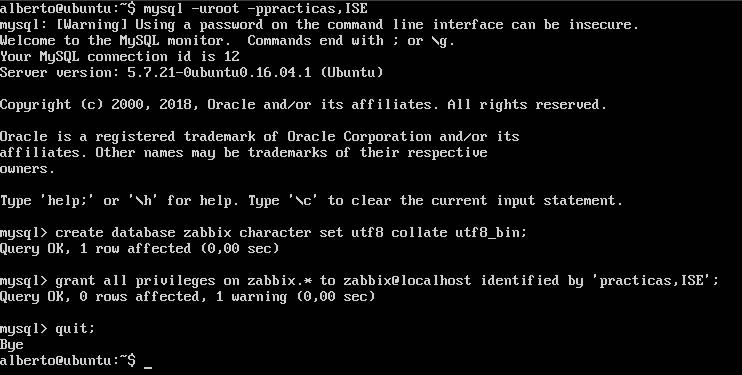
\includegraphics[scale=0.5]{images/bye.png}
 	\caption{Base de datos configurada}
 \end{figure}
 
 
 Ahora que la tenemos configurada, importamos los datos: \\
  \# \textit{zcat /usr/share/doc/zabbix-server-mysql/create.sql.gz $|$ mysql -uzabbix -p zabbix
  	}  \\ 
  
  
\newpage
 Configuramos la base de datos creada para el servidor. Para ello, debemos editar el archivo de configuración \textbf{zabbix\_server.conf} ubicado en /etc/zabbix/. 
 
\# \textit{vi /etc/zabbix/zabbix\_server.conf \\
DBHost=localhost \\
DBName=zabbix \\
DBUser=zabbix \\
DBPassword=practicas,ISE} \\

\begin{figure}[h]
	\centering
	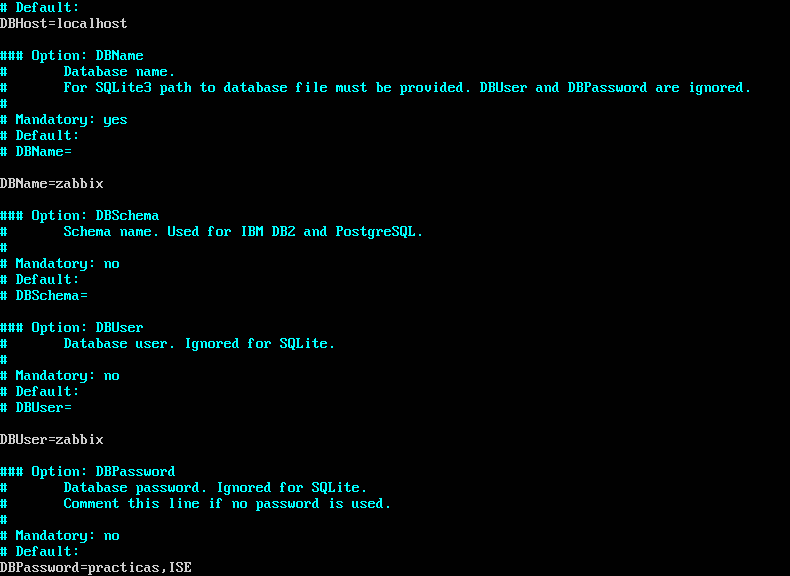
\includegraphics[scale=0.5]{images/4.png}
	\caption{/etc/zabbix/zabbix\_server.conf}
\end{figure}


\subsection{Iniciamos el servidor}

El siguiente paso a realizar será iniciar el servidor de Zabbix: \\
\# \textit{service zabbix-server start} \\
\# \textit{update-rc.d zabbix-server enable}\\

\newpage
Reiniciamos Apache: \\
\# \textit{service apache2 restart} \\

 \begin{figure}[h]
 	\centering
 	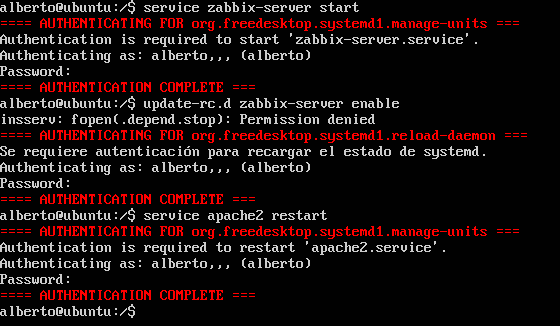
\includegraphics[scale=0.5]{images/2.png}
 	\caption{Servicios}
 \end{figure}
 
 


Es recomendable que modifiquemos el archivo  de la configuración de apache /etc/apache2/conf-enabled/zabbix.conf , descomentando la línea 'date.timezone' y establecer nuestra zona horaria, que se puede consultar en \url{http://php.net/manual/en/timezones.php} 

\# \textit{vi /etc/apache2/conf-enabled/zabbix-conf \\
	php\_value max\_execution\_time 300 \\
	php\_value memory\_limit 128M \\
	php\_value post\_max\_size 16M \\
	php\_value upload\_max\_filesize 2M \\
	php\_value max\_input\_time 300 \\
	php\_value always\_populate\_raw\_post\_data -1 \\
	\# php\_value date.timezone Europe/Riga} \\



 

Tenemos instalado el servidor en Ubuntu Server, sin embargo, es necesario instalar \\ también el agente: \\
\# \textit{apt-get install zabbix-agent} \\

Como es un servicio, lo tenemos que habilitar: \\
\# \textit{service zabbix-agent start} \\ 


Ahora comprobamos:
\textbf{http://192.168.56.105/zabbix}

\newpage
 \begin{figure}[h]
 	\centering
 	
\includegraphics[scale=0.5]{images/zabbix.png}
 	\caption{Base de datos configurada}
 \end{figure}
 

\subsection{Primer problema encontrado}
Cuando intentaba conectarme a la dirección \textit{192.168.56.105/zabbix} me daba un mensaje de error. Para solucionarlo he seguido los siguientes pasos:

\begin{itemize}
	\item Compruebo que tengo conexión entre el host y ubuntu con:\\ \#\textit{ping 192.168.56.1}
	\item Compruebo la conexión de zabbix con el comando: \\ \#\textit{curl localhost/zabbix}
	\item Como el protocolo \textbf{http} tiene el puerto 80, lo habilitamos: \\ \#\textit{ufw allow 80}
	\item Volvemos a comprobar conectarnos a la dirección y vemos que el problema ya ha sido solucionado
\end{itemize}


\newpage
\subsection{Configuración del frontend}

\begin{itemize}
	\item Comprobamos que todos los prerequisitos se cumplen
	\item Configuramos la conexión a la base de datos, para ello la base de datos debe estar creada
	\item Rellenamos los detalles del servidor
	\item Comprobamos que los datos introducidos son correctos:
	
	 \begin{figure}[h]
	 	\centering
	 	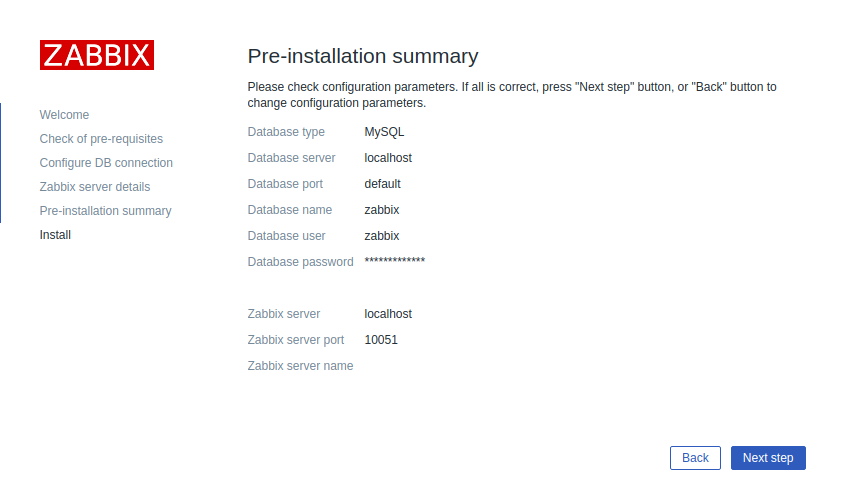
\includegraphics[scale=0.5]{images/summary.png}
	 	\caption{Configuración frontend}
	 \end{figure}
	
\end{itemize}

\newpage
Si hemos configurado correctamente Ubuntu Server y CentOS, realizaremos los siguiente pasos:


\begin{itemize}
	\item Desde el frontend, nos dirigimos a \textit{Configuration/Host} y añadimos lo siguiente:
	 \begin{figure}[h]
	 	\centering
	 	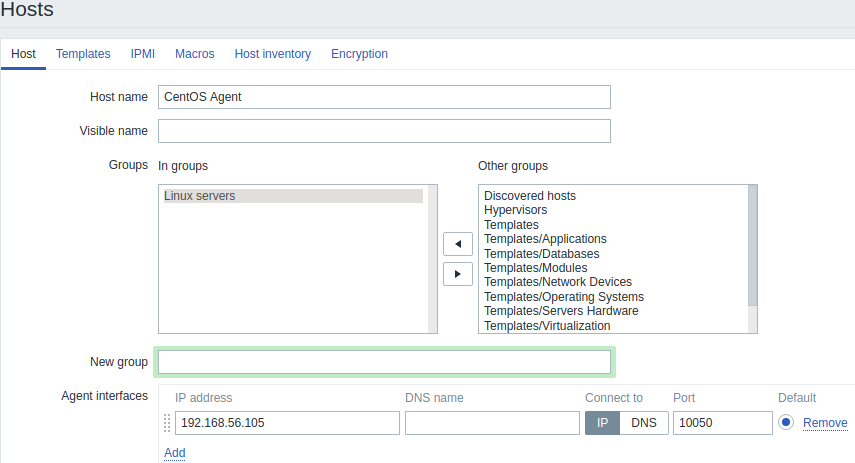
\includegraphics[scale=0.4]{images/cent.png}
	 	\caption{Nuevo host CentOS}
	 \end{figure}
	
	\item En la pestaña \textit{templates}, añadimos:
	\begin{figure}[h]
		\centering
		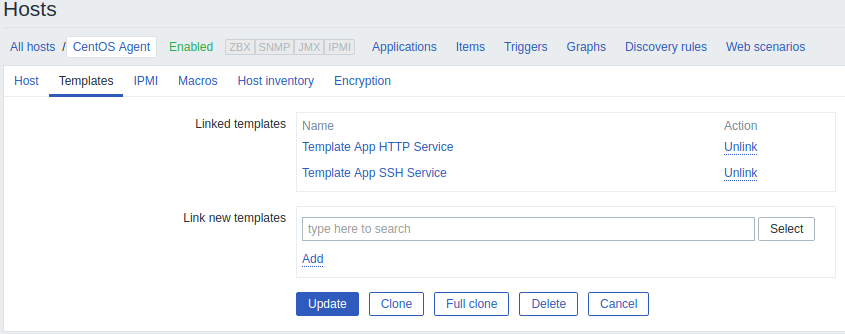
\includegraphics[scale=0.45]{images/biencent.png}
		\caption{Templates centOS}
	\end{figure}
	\item Hacer lo mismo para Ubuntu Server. En esta caso el proceso es igual ya que los procesos a monitorizar son los mismos, \textbf{ssh} y \textbf{http}.Lo únicamente que tendremos que cambiar son:
	
	\begin{itemize}
		\item El nombre del host: Ubuntu Server and Agent
		\item IP: 127.0.0.1 , ya que utiliza la misma IP que el servidor
	\end{itemize}
	
	
\end{itemize}



Si todo ha ido correctamente, tendremos:
\begin{figure}[h]
	\centering
	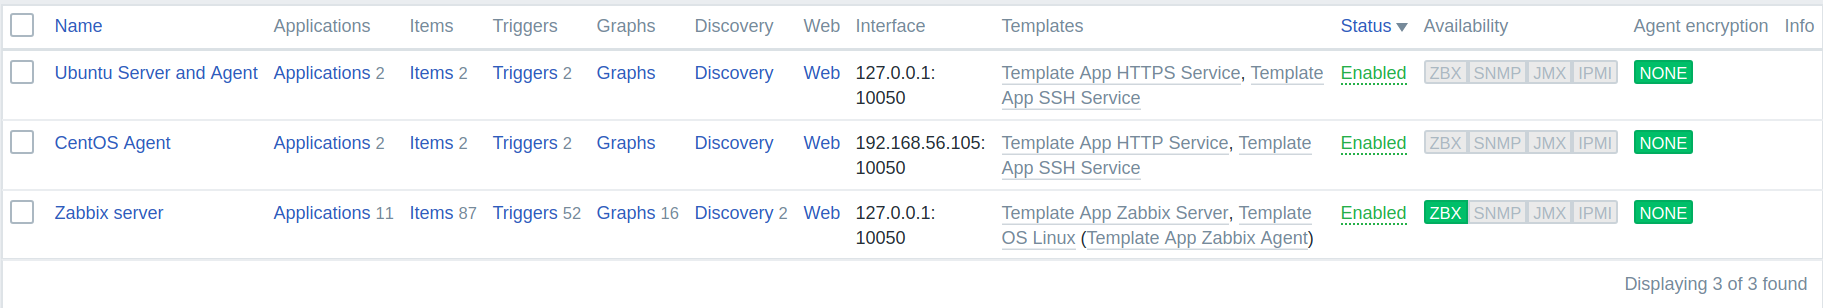
\includegraphics[scale=0.26]{images/bieen.png}
	\caption{Templates frontend}
\end{figure}

Nos dirigimos a la pestaña \textit{Monitoring/DashBoard} y nos encontramos el siguiente error:

\begin{figure}[h]
	\centering
	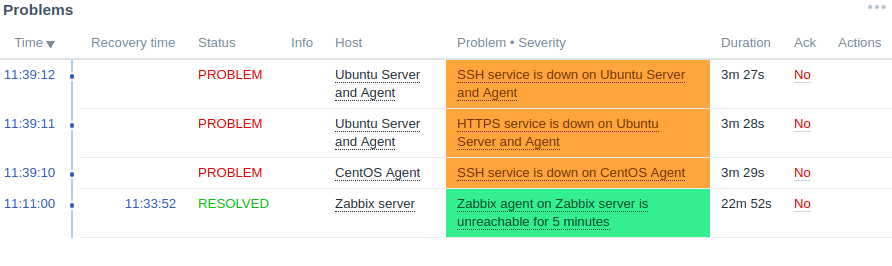
\includegraphics[scale=0.45]{images/error.png}
		\caption{Error en los servicios}
\end{figure}

Si comprobamos la captura anterior, vemos que hemos introducido el servicio \textit{HTTPS} en lugar de \textit{HTTP} por lo que para solucionarlo, cambiamos dicho servicio en la pestaña de templates. \\
Por otro lado, los servicios están inactivos por lo que los habilitamos: \\
\# \textit{systemctl restart sshd} \\

Por último, como usamos el puerto 22022 para ssh, cambiamos dicho puerto en el item del template

\begin{figure}[h]
	\centering
	
\includegraphics[scale=0.5]{images/a.png}
	%caption{Configuración agente}
\end{figure}

\newpage
\subsection{Revisión de errores}


En caso de aparecer un mensaje de conexión inválida, podemos ver los logs del proceso en \textit{/var/log/zabbix}, tanto en Ubuntu Server como en centOS


\begin{figure}[h]
	\centering
	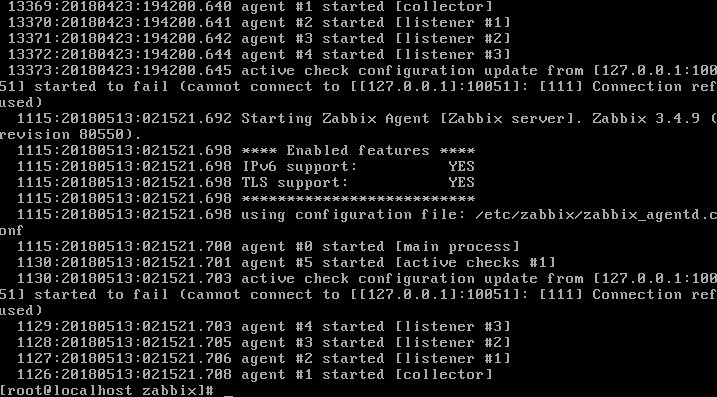
\includegraphics[scale=0.4]{images/b.png}
	\caption{/var/log/zabbix/zabbix\_agentd.log}
\end{figure}

El problema anterior se ha solucionado introduciendo la ip correcta en los archivos de configuración de zabbix.

Para probar que el proceso ha finalizado correctamente, podemos hacerlo con la orden:
\# \textit{zabbix\_get -s 'dirIP' -k net.tcp.service['Service name']} \\
que previamente hemos instalado tanto en centOS como en Ubuntu Server \\

\textbf{Ubuntu Server}: 
\begin{itemize}
	\item sudo apt-cache search zabbix \\
	 sudo apt-get install zabbix-get
\end{itemize} 

\textbf{CentOS}
\begin{itemize}
	\item yum search zabbix-get \\ yum install zabbix-get.x86\_64
\end{itemize} 


\begin{figure}[h]
	\centering
	
\includegraphics[scale=0.5]{images/final.png}
	\caption{Ubuntu server: Zabbix\_get}
\end{figure}

\begin{figure}[h]
	\centering
	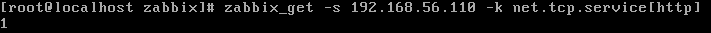
\includegraphics[scale=0.5]{images/final2.png}
	\caption{CentOS: Zabbix\_get}
\end{figure}

\newpage
Por otro lado, también hemos probado que zabbix funciona correctamente parando y reiniciando el servicio de la forma:

\begin{figure}[h]
	\centering
	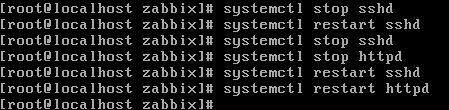
\includegraphics[scale=0.5]{images/bateria.png}
	\caption{Prueba de comandos}
\end{figure}

\begin{figure}[h]
	\centering
	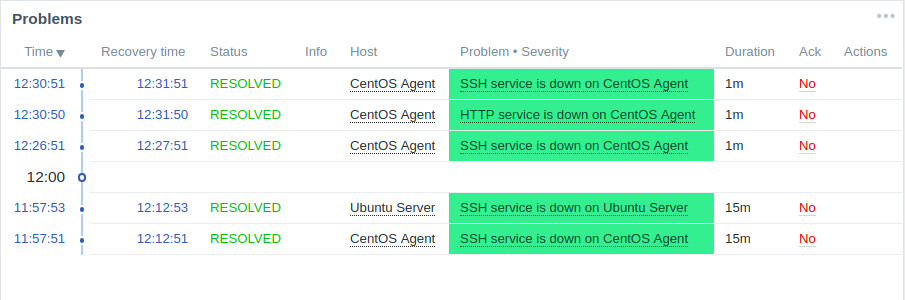
\includegraphics[scale=0.5]{images/final3.png}
	\caption{Zabbix - Correcto funcionamiento}
\end{figure}



\newpage
\section{CentOS}

En CentOS únicamente tendremos que instalar el agente por lo que no tenemos que instalar una base de datos

\subsection{Instalación}

Nos descargamos el siguiente repositorio:

\# \textit{rpm -ivh http://repo.zabbix.com/zabbix/3.4/
	rhel/7/x86\_64/zabbix-release-3.4-2.el7.noarch.rpm} \\


Instalamos el agente de Zabbix: \\
\# \textit{yum install zabbix-agent} \\



Si probamos a iniciar el agente nos dará error, por lo que haremos lo siguiente: \\
\# \textit{cat /var/log/audit/audit.log | grep zabbix\_agentd | grep denied |
	audit2allow -M zabbix\_agent\_setrlimit} 

\# \textit{semodule -i zabbix\_agent\_setrlimit.pp} \\

\# \textit{systemctl restart zabbix-agent} \\


\begin{figure}[h]
	\centering
	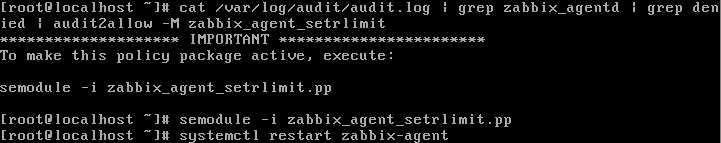
\includegraphics[scale=0.5]{images/next.png}
	%caption{Configuración agente}
\end{figure}


Ahora ya podemos iniciar el agente sin problemas: \\
\# \textit{systemctl start zabbix-agent} \\
\# \textit{systemctl status zabbix-agent} \\

\begin{figure}[h]
	\centering
	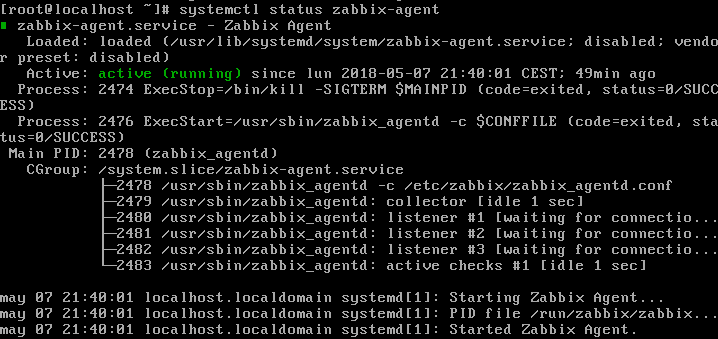
\includegraphics[scale=0.5]{images/next2.png}
	%\caption{Zabbix-agent iniciado correctamente}
\end{figure}




%para firefox usar 'RESTED', en 'POST' ponemos la url de "zabbix...jsonrpc.php"


\newpage
\begin{thebibliography}{9}
	\bibitem{Zabbix Documentation} 
	Zabbix Documentation,
	\\\texttt{https://www.zabbix.com/documentation/3.4/manual/installation}
	
	\bibitem{Ubuntu Server} 
	Ubuntu Server,
	\\\texttt{https://www.zabbix.com/documentation/3.4/manual/installation/install\_from\_packages\\/debian\_ubuntu}
	
	\bibitem{CentOS} 
	CentOS,
	\\\texttt{https://www.zabbix.com/documentation/3.4/manual/installation/install\_from\_packages\\/rhel\_centos}
	
\end{thebibliography}



\end{document}